%%%%%%%%%%%%%%%%%%%%%%%%%%%%%%%%%%%%%%%%%
% Formal Text-Rich Title Page 
% LaTeX Template
% Version 1.0 (27/12/12)
%
% This template has been downloaded from:
% http://www.LaTeXTemplates.com
%
% Original author:
% Peter Wilson (herries.press@earthlink.net)
%
% License:
% CC BY-NC-SA 3.0 (http://creativecommons.org/licenses/by-nc-sa/3.0/)
% 
% Instructions for using this template:
% This title page compiles as is. If you wish to include this title page in 
% another document, you will need to copy everything before 
% \begin{document} into the preamble of your document. The title page is
% then included using \titleGP within your document.
%
%%%%%%%%%%%%%%%%%%%%%%%%%%%%%%%%%%%%%%%%%

%----------------------------------------------------------------------------------------
%	PACKAGES AND OTHER DOCUMENT CONFIGURATIONS
%----------------------------------------------------------------------------------------

\documentclass{article}
\usepackage{graphicx}
\newcommand*{\plogo}{\fbox{{Fortran}}} % Generic publisher logo
\usepackage[spanish]{babel}
\usepackage{epsfig,graphics,fancyvrb}
%----------------------------------------------------------------------------------------
%	TITLE PAGE
%----------------------------------------------------------------------------------------

\newcommand*{\titleGP}{\begingroup % Create the command for including the title page in the document
\centering % Center all text
\vspace*{\baselineskip} % White space at the top of the page

\rule{\textwidth}{1.6pt}\vspace*{-\baselineskip}\vspace*{2pt} % Thick horizontal line
\rule{\textwidth}{0.4pt}\\[\baselineskip] % Thin horizontal line

{\LARGE Departamento \\% OF \\[0.3\baselineskip] \LaTeX
 ~de F\'isica}\\[0.2\baselineskip] % Title

\rule{\textwidth}{0.4pt}\vspace*{-\baselineskip}\vspace{3.2pt} % Thin horizontal line
\rule{\textwidth}{1.6pt}\\[\baselineskip] % Thick horizontal line

\scshape % Small caps
\Large{\textbf{Ciencias Exactas Y Naturales}\\ % Tagline(s) or further description
\textbf{Programaci\'on y Lenguaje Fortran}}\\[\baselineskip] % Tagline(s) or further description
\par % Location and year
\vspace*{1\baselineskip}
Compiladores e Interpretadores \\ Para diferentes lenguajes de programaci\'on

\vspace*{2\baselineskip} % Whitespace between location/year and editors

%Hecho por \\[\baselineskip]
{\Large Sandra Yulissa M\'endez Parra\par} % Editor list
\vspace*{1\baselineskip}
{\itshape Universidad de Sonora\\ Mex.\par} % Editor affiliation

{
\setlength{\unitlength}{1 cm} %Especificar unidad de trabajo
\thispagestyle{empty}
\begin{picture}(0,0)
\put(2,8.9){
\includegraphics[width=2cm,height=2cm]{logo.jpeg}}
%\put(11.5,0){\includegraphics[width=4cm,height=4cm]{eupinf.jpg}}
\end{picture}}

\vfill % Whitespace between editor names and publisher logo

\plogo \\[0.3\baselineskip] % Publisher logo
{\scshape Hermosillo, Sonora 2015} \\[0.3\baselineskip] % Year published


\endgroup}

%----------------------------------------------------------------------------------------
%	BLANK DOCUMENT
%----------------------------------------------------------------------------------------

\begin{document} 

\pagestyle{empty} % Removes page numbers

\titleGP % This command includes the title page
\newpage

En la siguiente tabla se ver\'an los compiladores e interpretadores para dieferentes lenguajes de programaci\'on. \linebreak \linebreak
{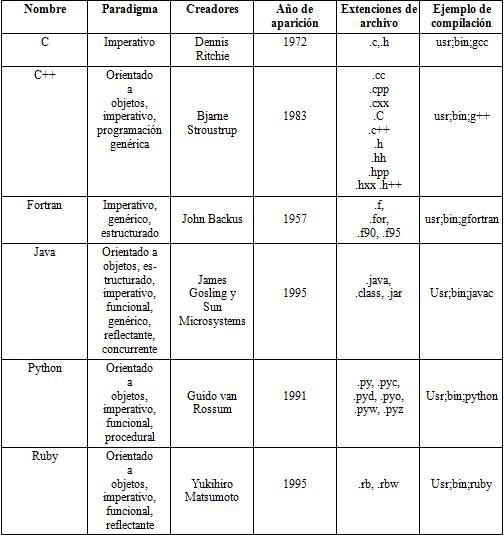
\includegraphics[width=1\textwidth]{123.jpg}}

C
\begin{verbatim}
#include <stdio.h>
int main()
{printf("¡Hola, mundo!");
return 0;}
\end{verbatim}

C++
\begin{verbatim}
#include <iostream>
using namespace std;
int main()
{
cout<<"¡Hola mundo!";
return 0 ;
}
\end{verbatim}


Fortran
\begin{verbatim}
PROGRAM HOLA
PRINT *, ’¡Hola, mundo!’
END
\end{verbatim}
Java
\begin{verbatim}
public class HolaMundo
{public static void main(String[] args)
{System.out.println("Hola Mundo");}}
\end{verbatim}


Python
\begin{verbatim}
print ("Hola Mundo")
\end{verbatim}

Ruby
\begin{verbatim}
puts "Hola Mundo"
\end{verbatim}

\end{document}
